\documentclass[a4paper,man,natbib]{apa6}

\usepackage[english]{babel}
\usepackage[utf8x]{inputenc}
\usepackage{amsmath}
\usepackage{graphicx}
\usepackage[colorinlistoftodos]{todonotes}


% specify link style
\usepackage{hyperref}
\hypersetup{
    colorlinks=true,
    linkcolor=blue,
    filecolor=magenta,      
    urlcolor=cyan,
    citecolor=blue
}

% override apa6 section headers
% https://tex.stackexchange.com/questions/125537/how-to-modify-subsubsection-header-apa6-cls
\makeatletter
\renewcommand{\subsubsection}{\@startsection{subsubsection}{3}
  {\z@}%
  {\b@level@two@skip}{\e@level@two@skip}%
  {\normalfont\normalsize\bfseries}}
\makeatother

% override apa6 first paragraph index
% https://tex.stackexchange.com/questions/155028/indentation-apa6-class-for-2nd-paragraphs-after-title
% \makeatletter
%   \b@level@one@skip=-2.5ex plus -1ex minus -.2ex
%   \b@level@two@skip=-2.5ex plus -1ex minus -.2ex
% \makeatother

\title{An item response theory analysis of the Matrix Reasoning Item Bank (MaRs-IB)}
\shorttitle{IRT analysis of MaRs-IB}
\author{Samuel Zorowitz$^1$, Nathaniel D. Daw$^{1,2}$}
\affiliation{$^1$Princeton Neuroscience Institute, Princeton University, USA\\$^2$Department of Psychology, Princeton University, USA}

\abstract{Your abstract here.}

\begin{document}
\maketitle

\section{Introduction}

Matrix reasoning tasks are among the most widely used measures of cognitive ability in the behavioral sciences. Much of their popularity undoubtedly reflects their versatility in use. Matrix reasoning tasks are strong (albeit impure) indicators of general intelligence \citep{gignac2015raven} and working memory capacity \citep{kane2004generality, unsworth2005working}. They are predictive of important real-world outcomes such as childhood academic performance \citep{roth2015intelligence} and performance on college entrance exams \citep{frey2004scholastic, koenig2008act}. In low-stakes testing settings, matrix reasoning tasks can additionally function as measures of motivation, willingness to expend mental effort, and other aspects of personality \citep{duckworth2011role, gignac2019maximum}. Performance on matrix reasoning tasks can also serve as an instrumental variable in studies of psychiatric populations; that is, it can be used to control for general disruptions to cognitive ability where specific domains of cognition are primarily of interest \citep{gillan2016characterizing, rouault2018psychiatric, moutoussis2021decision}.

Unfortunately there are a number of impediments to using matrix reasoning tasks as part of behavioral research. One such challenge is the problem of copyright. The most prominent examples of matrix reasoning tasks, such as Raven's progressive matrices \citep{raven2003raven} and the WAIS matrix subtest \citep{wechsler1999wechsler}, are not free to use and have legal restrictions against being computerized. A second challenge is that, across all of the matrix reasoning tests in the public domain, there are relatively few unique items available. The Hagen matrices test \citep{heydasch2014hagen} and ICAR matrix reasoning test \citep{condon2014international}, for example, have only 20 and 16 items respectively. The availability of only a limited number of items raises the possibility of repeat exposure effects, which threaten the validity of these measures  \citep{ng1974applicability, bors2003effect}. This problem is exacerbated in the current age of online experiments, where multiple groups of researchers may be unintentionally administering the same test to the same participants recruited from the same online labor platforms.

Noting these challenges, \cite{chierchia2019matrix} developed and made publicly available the matrix reasoning item bank (MaRs-IB), a collection of 80 unique matrix reasoning puzzles. Each puzzle in the MaRs-IB consists of a 3x3 matrix containing abstract shapes in eight out of nine cells (Figure \ref{fig:fig00}). To solve a puzzle, participants must deduce which of four response options correctly completes the matrix based on the pattern of changing relations among the shapes across cells. The puzzles in the MaRs-IB were designed to span a considerable range of complexity, both in the number of unique shapes and changing relations in and across cells. To further increase the reusability of the MaRs-IB and minimize practice effects, each puzzle (hereafter referred to as a template item) has six clones. An item's clones share identical structural properties (i.e. number of shapes, number of changing relations) but may vary in their distractors (two unique sets per item) or perceptual features (three unique shape sets per item). Thus, the MaRs-IB addresses several issues associated with other matrix reasoning tests.   

\cite{chierchia2019matrix} also conducted an initial study of the psychometric properties of the MaRs-IB. A sample of 659 participants completed a fixed-length and fixed-order test measure in which they had eight minutes to complete as many MaRs-IB items as possible. The authors found that performance on this test measure had good split-half and test-retest reliability. Moreover they found that participants' ability to solve puzzles in the MaRs-IB was moderately predictive of their performance on a digit span task and the ICAR matrix reasoning test, indicating good convergent validity. At the conclusion of this study, \cite{chierchia2019matrix} publicly released a summary of the difficulty (i.e. proportion correct responses) of each item in the MaRs-IB so that future researchers could construct new test measures of custom difficulty and duration.

Unfortunately, there are two critical limitations in this study that undermine the utility of the summary statistics. The first is that, given design of the test, there was relatively little data collected for the majority of the items in the MaRs-IB. Indeed, only half (42 of 80 items) were completed by 100 or more participants. As such, one cannot be confident about the reported functioning of a majority of the items (an issue that is exacerbated when considering that each item has six clones). A second issue is participants were allowed to choose for themselves whether to prioritize accuracy (number of correct responses) or productivity (number of items reached). As a consequence, the response data for items that came later in the fixed-order test were increasingly likely to be produced by participants sacrificing accuracy for speed, thereby biasing the proportion correct measure for these items (see the Supplementary materials for evidence of this point). Therefore, additional investigation of the functioning and psychometric properties of the MaRs-IB is warranted.

Here we provide a more extensive study and psychometric validation of the MaRs-IB. The most important contribution of the current work is the characterization of (almost) every item in the MaRs-IB using item response theory (IRT) \citep{embretson2013item, de2013theory}. IRT models confer several important advantages for the purposes of psychometric validation. First they provide an estimate of the difficulty and discrimination of each item, where the latter is an index of how much information an item provides given a level of ability. Using these quantities, IRT models in turn facilitate the computation of the test information function (TIF), which measures the reliability of a test measure across a range of ability. Finally, IRT models make possible optimal test assembly  \citep{van1998optimal}, or the design of new tests with maximal reliability given researcher-specified constraints (e.g. test duration, test difficulty).

A second contribution provided here is an investigation of the relationship between the attributes of MaRs-IB items and their psychometric properties using explanatory item response models \citep{de2004explanatory, wilson2008explanatory}. The utility of the MaRs-IB depends in part on its items exhibiting certain expected characteristics. Across items we should expect complexity (e.g. more shapes per cell, more changing relations) to be positively associated with difficulty. Moreover if item clones are exchangeable (i.e. perfect replicas with identical psychometric properties), then we should expect no association between distractor type and difficulty. Thus explanatory IRT models offer an opportunity to evaluate the success of the MaRs-IB design. As a secondary benefit, explanatory IRT models also provide more accurate estimates of item parameters \citep{neuhaus2006separating}. 

A third contribution is the decomposition of variance in item functioning, into modeled and unmodeled sources, using additive multilevel item structure (AMIS) models \citep{geerlings2011modeling, cho2014additive, lathrop2017item}. First we use AMIS models to quantify the residual variance in difficulty and discrimination across items after accounting for their respective attributes. At the item-level, smaller residual variances indicate that items are functioning as intended. We also use AMIS models to quantify the variance in difficulty and discrimination across item clones. If item clones are to be treated as exchangeable (i.e. able to be used interchangeably), then the residual variance in their item parameters must be negligible. AMIS models therefore provide a second means by which to evaluate the success of the MaRs-IB design.

The remainder of the paper proceeds as follows. First we report a calibration study, in which a large sample of participants each completed a subset of items from the MaRs-IB. Using their response data, we then fit a series of multilevel item structure models in order to estimate item parameters for each item (and their clones). Using these same models, we also interrogate the relationship between item attributes and functioning within and cross items in the MaRs-IB. Then we report a second validation study, in which a smaller sample of participants completed one of three new MaRs-IB short-form tests. These tests --- designed using optimal test assembly methods applied to the item parameters estimated during the calibration study --- were found to have good psychometric properties and convergent validity. This second study provides a blueprint for how to construct new MaRs-IB test measures using the item parameter estimates that have been released as part of this study.

All data, code, and model outputs (including the item parameter estimtes) are publicly available at: \url{https://github.com/dawlab/mars-irt}.

\clearpage
\section{Calibration Study}

\subsection{Objectives}

The purpose of the first study was to calibrate the items of the MaRs-IB using response data collected from a large number of adult participants from the general population. In particular, we sought to accomplish the following three objectives: (1) to characterize the psychometric properties of the items in the MaRs-IB using item response models; (2) to investigate the associations between item attributes and their psychometric properties, and (3) to determine the equivalence of items with similar complexities, and clones of the same item templates. 

\subsection{Methods}

\subsubsection{Participants} 

A total of N=1584 participants were recruited from the Prolific Academic platform (\url{https://www.prolific.co}) to participate in an online experiment between July - August, 2021. Participants were eligible if they were 18 years or older and lived in the United States. Total study duration was approximately 6.4 minutes (sd = 2.4) per participant. Participants received monetary compensation for their time (rate: \$10 USD/hr), plus a performance-based bonus up to \$0.50 USD. On average, participants earned a total of \$1.30 USD (sd = \$0.10). We offered performance bonuses as they have been found to motivate performance in low-stakes testing environments \citep{duckworth2011role, gignac2018moderate}. This study was approved by the Institutional Review Board of Princeton University (\#7392), and all participants provided informed consent.

To ensure data quality, the data from multiple participants were excluded prior to analysis (see Exclusion Criteria below) leaving the data from N=1501 participants for analysis. In these participants, the majority identified as women (men: N=670; women: N=811; non-binary or other: N=13; rather not say: N=2) and the average age was 28.7 years old (sd = 9.9). The sample was relatively well-educated with the majority having completed a Bachelor's degree (N=507) or Master's degree or higher (N=322). Comparatively fewer participants completed only some college (N=471), only a high school degree (N=199), or preferred not to say (N=2). 

\subsubsection{Procedure}

After providing consent, participants completed 16 items from the MaRs-IB. The design of the MaRs-IB items have been described previously \citep{chierchia2019matrix}. Briefly, each MaRs-IB item consists of a 3 x 3 matrix. Eight of the nine resulting cells contain abstract shapes, while one cell on the bottom right-hand side of the matrix is empty. Participants are instructed to ``complete the matrix'' by identifying the missing shape from among four possible alternatives. 

The presentation of each item was preceded by a fixation cross, which lasted for 1200 ms. Upon presentation of the item, participants were given up to 30 s to solve the puzzle. After 25 s elapsed, a clock appeared to count down the remaining 5 s. A trial ended when participants responded, or after 30 s had elapsed without response. Before the trials began, participants reviewed instructions and were made to correctly complete three practice items. Participants were instructed to respond carefully, but to guess if they could not solve the puzzle before the timer ran out. The format of the experiment and instructions were adapted from code publicly released as part of the original study (\url{https://app.gorilla.sc/openmaterials/36164}).

In order to ensure sufficient sampling of every item (and their clones) in the MaRs-IB, participants were administered a pseudorandomly-selected set of 16 out of 64 total items.\footnote{We did not collect new data for the 16 easiest items in the MaRs-IB (items 1, 2, 3, 4, 5, 7, 8, 9, 32, 33, 38, 41, 43, 48, 57, 68) because performance on these items was at or near ceiling.} Item sets were constructed as follows: We subdivided the 64 items into 16 sets of four based on their dimensionality (a measure of item complexity defined in \cite{chierchia2019matrix}). Participants were randomly assigned one item from each of the 16 sets. As a consequence, all participants received test forms of roughly equal difficulty. Importantly we also counterbalanced the assignment of item clones across participants, such that we had an approximately uniform number of responses available for each item by shape set (1, 2, or 3) and distractor type (minimal difference, MD, or or paired difference, PD; see \cite{chierchia2019matrix} for details). 

\subsubsection{Exclusion criteria}

The data from multiple participants who completed the experiment were excluded prior to analysis for one or more of the following reasons: rapid guessing (responding in less than 3 s) on four or more trials (N=70); failing to respond on four or more trials (N=8); or minimizing the browser window to a dimension smaller than the minimal requirements (N=7). In total, 83 of 1584 (5.2\%) participants were excluded leaving the data from N=1501 participants available for analysis. Across these participants, each item (64 total) was administered approximately 375 times (sd = 12) and each item clone (384 total) was administered approximately 62 times (sd = 7). 

\subsubsection{Item response models}

We employed item response models to characterize the psychometric properties of each item. Specifically, we used additive multilevel item structure (AMIS) models \citep{geerlings2011modeling, cho2014additive, lathrop2017item}. In AMIS models, item parameters are defined according to a hierarchical structure in which clones descend from item templates. At the core of of all of the AMIS models used here is the three parameter logistic (3PL) item response model, where the probability of a correct response ($y_{ijk} = 1$) for person $i$ on item clone $k$ belonging to item template $j$ is:

\begin{equation} \label{eq:1}
p(y_{ijk} = 1) = \gamma_{jk} + (1-\gamma_{jk}) \cdot \text{logit}^{-1} \left( \alpha_{jk} \cdot \theta_i - \beta_{jk} \right)
\end{equation}

\noindent where $\theta_i$ is the latent ability for person $i$, and $\beta_{jk}$, $\alpha_{jk}$, and $\gamma_{jk}$ are the difficulty, discrimination, and guessing parameters for item clone $k$ of item family $j$. Because the estimates of guessing parameters are often unreliable in the absence of very large amounts of data \citep{han2012fixing}, we fixed the guessing parameter for every item clone to the nominal guessing rate ($\gamma_{jk} = 0.25$).

The difficulty and discrimination parameters were estimated following an additive multilevel item structure. Concretely, the difficulty of item clone $k$ belonging to item template $j$ was expressed as:  

\begin{equation}
\beta_{jk} = \mu_\beta + \sum_{n=1}^N Q_{jn} \delta_{\beta n} + \epsilon_{\beta j} + \sum_{m=1}^M R_{km} \delta_{\beta m} + \epsilon_{\beta k}
\end{equation}

\noindent such that each item difficulty parameter was modeled as an intercept ($\mu_\beta$), reflecting the average difficulty across all items, and four additional components:

\begin{enumerate}

\item $\sum_{n=1}^N Q_{jn} \delta_{\beta n}$: the effect of the template (level 1) attributes on item difficulty, where $Q_{jn}$ is the value of attribute $n$ for item template $j$, and $\delta_{\beta n}$ is the effect of attribute $n$. 

\item $\epsilon_{\beta j}$: the template (level 1) residual, or residual variability in item difficulty of the item template unexplained by its attributes.

\item $\sum_{m=1}^M R_{km} \delta_{\beta m}$: the effect of the clone (level 2) attributes on item difficulty, where $R_{km}$ is the value of attribute $m$ for item clone $k$, and $\delta_{\beta m}$ is the effect of attribute $m$. 

\item $\epsilon_{\beta k}$: the clone (level 2) residual, or residual variability in item difficulty of the item clone unexplained by its attributes.

\end{enumerate}

\noindent In turn, item discrimination parameters were expressed as the sum of an equivalent set of components:

\begin{equation}
\alpha_{jk} = \mu_\alpha + \sum_{n=1}^N Q_{jn} \delta_{\alpha n} + \epsilon_{\alpha j} + \sum_{m=1}^M R_{km} \delta_{\alpha m} + \epsilon_{\alpha k}
\end{equation}

\noindent where the interpretation of each component is the same as for item difficulty.

In our analyses, we considered two template level (level 1) attributes: feature number, or the number of elements in each cell of an item; and rule number, or the number of changing relationships across the cells of an item (e.g. color change, shape change, position change). We predicted that both attributes would be positively associated with item difficulty; that is, all else equal, items with a great number of features or rules would be more difficult to solve. In contrast, we had no hypotheses about the relationship between these attributes and item discrimination. 

We also considered two clone level (level 2) attributes: distractor type, or the use of MD-type versus PD-type response alternatives; and mean response time, or the average time participants spent deliberating on that item clone. We note that, in contrast to all other modeled attributes, average response time is not an intrinsic property of an item. We opted to include it in our models, however, because including response time as a covariate has previously been shown to improve parameter estimation \citep{bertling2018using}. To prevent possible collinearity between the attributes, mean response time was orthogonalized with respect to the three other item attributes; therefore, any effects of response time reflects residual structure after accounting for all other item attributes. Based on \cite{chierchia2019matrix}, we predicted there would be no association between distractor type and item difficulty, and a positive association between mean response time and item difficulty. As with the template-level attributes, we had no hypotheses about the relationship between the clone-level attributes and item discrimination. 

The AMIS model framework provides a natural means of accomplishing the three goals of the calibration the study. By fitting an AMIS model, we estimate the item parameters and quantify the psychometric properties for every item, and their clones, in the MaRs-IB (Aim 1). By modeling the effects of item attributes, we can evaluate the success of the MaRs-IB design by investigating whether item attributes influence item functioning as expected (e.g. a positive association between rule number and item difficulty; Aim 2). Finally, by estimating the magnitude of residual error in item parameters from unmodeled sources of variance (e.g. perceptual features), we can test whether the MaRs-IB possesses certain desirable structural properties (e.g. psychometric equivalence and exchangeability among item clones; Aim 3). 

We also estimated person-level abilities following an explanatory item response modeling approach \citep{wilson2008explanatory}: 

\begin{equation} \label{eq:4}
\theta_i = \sum_{p=1}^P X_{ip} \rho_p + \epsilon_i    
\end{equation}

\noindent where $X_{ip}$ is the value of attribute $p$ for person $i$, $\rho_p$ is the partial correlation of attribute $n$, and $\epsilon_i$ is variance in ability unexplained by the person-level attributes. 

We investigated person-level abilities as a function of four covariates: age, gender, average response time, and $\Delta$ response time. This last term reflects the degree of change in a participant's deliberation time as a function of item difficulty (defined as one minus the proportion of correct responses for that item). All covariates were standard-scored prior to analysis with the exception of gender, which was binary coded (male = -0.5, female = 0.5).

\subsubsection{Model Fitting}

All models were estimated within a Bayesian framework using Hamiltonian Monte Carlo as implemented in Stan (v2.22) \citep{carpenter2017stan}. For all models, four separate chains with randomised start values each took 7500 samples from the posterior. The first 5,000 samples from each chain were discarded. As such, 10,000 post-warmup samples from the joint posterior were retained. The $\hat{R}$ values for all parameters were equal to or less than 1.01, indicating acceptable convergence between chains, and there were no divergent transitions in any chain. 

During estimation, the item discrimination parameters were restricted to be in the range $\alpha_{jk} \in [0, 5]$. To ensure the identifiability of all models, person abilities were constrained to have a mean of zero and a variance of 1.0. In other words, the residual variance in ability was specified as $V(\epsilon) = 1 - \sum \rho_p^2$.

\subsubsection{Model comparison}

The goodness of fit of the models was compared using Bayesian leave-one out cross-validation \citep{vehtari2017practical}, which has been found to perform better than more traditional information criteria for comparing item response models \citep{luo2017performances}. We computed the conditional leave-one-cluster out (LOCO) cross-validation \citep{merkle2019bayesian}, which measures a model's ability to generalize to held out items (rather than held out responses or held out participants) --- i.e., for inferring generalization to additional items constructed using the same features rather than to additional participants sampled from the same population.

\subsubsection{Goodness of fit}

The fit of the best-fitting model to the data was evaluated using posterior predictive model checking \citep{gelman1996posterior, levy2017bayesian}. A sample of predicted responses was generated for each sample of item parameters and the posterior predictive $p$ (PPP) value was computed based on two discrepancy statistics:  the Orlando and Thissen index ($S-\chi^2$) \citep{toribio2011discrepancy} and the standardized generalized dimensionality discrepancy measure (SGDDM) \citep{levy2015standardized}. 

The $S-\chi^2$ discrepancy statistic is a measure of item fit based on the comparison of observed and expected proportions of examinees who answer an item correctly at each raw-score group. A global measure of fit at the test level is obtained by summing the discrepancy values over the items. SGDDM is a measure of model dimensionality. More specifically, SGDDM may be interpreted as the mean absolute conditional correlation between all non-redundant pairs of items, which allows for the identification of inter-item correlations beyond those explained by the model. This latter measure is important as it tests for the presence of non-negligible response dependence across items, which may otherwise lower the efficiency of future test forms due to the inclusion of nonindependent or  redundant items.

\subsection{Results}

\subsubsection{Descriptive statistics}

On average, participants completed 9.6 of 16 items correctly (sd = 3.1, IQR = 8.0 -- 12.0) (Figure \ref{fig:fig01}a). Timing out occurred on only 1.8\% of trials. A total of 43 participants (2.9\%) performed below chance (i.e. fewer than four items correct), while only 11 participants (0.7\%) solved all 16 of their items. Thus, over 95\% of observed scores were in a reasonable range. These results corroborate those reported by \cite{chierchia2019matrix} in that there were no obvious ceiling or floor effects in performance, and that the majority of participants were sufficiently motivated to participate in spite of the low-stakes testing environment.  

Across all 384 item clones, the average proportion correct was 0.60 (sd = 0.19, IQR = 0.45 - 0.74; Figure \ref{fig:fig01}b). A total of 12 items (3.1\%) exhibited performance levels beneath chance, and only 22 items (5.7\%) had performance levels near ceiling ($\geq$ 90\%). Across items, the proportion of correct responses was negatively correlated with rule number ($\rho$ = -0.482, p < 0.001). These results further corroborate those reported by \cite{chierchia2019matrix} in that the MaRs-IB exhibited good functioning with performance levels for only a few item clones at ceiling or floor. 

We investigated the relationship between accuracy and response time using a mixed effects (random intercepts) linear regression model. Participants' log-transformed response times were predicted as a function of that trial accuracy, rest score (participants' observed scores on all other items), and item difficulty (one minus the proportion correct for that item). The mixed-effects model was estimated using the \textit{statsmodels} python package (v0.12.2) \citep{seabold2010statsmodels}).

The results are summarized in Table \ref{table:1}. On average, participants spent 15.9 s (sd = 7.2 s) on each item. There were significant main effects of accuracy ($\beta = 0.067$, $t = 9.84$, $p < 0.001$), rest score ($\beta = 0.125$, $t = 16.95$, $p < 0.001$), and item difficulty ($\beta = 0.137, t = 44.33, p < 0.001$). That is, response times were slower for correct responses, better-performing participants, and more difficult items.

There were also significant accuracy by difficulty and  accuracy by rest score interactions. Correct responses were even slower for more difficult items, but faster for better performing participants. There was also a significant difficulty by score interaction, such that better performing participants exhibited slower responses for more difficult items. This pattern of response time results is visible in Figure \ref{fig:fig01}c. The three-way interaction term was not significant. 

\subsubsection{Alternative item structure models}

We fit a series of nested AMIS models in order to identify the model that best predicted participants' response data. The models varied in how item parameters were specified, with each successive model allowing for greater flexibility in item parameter estimation. For the goals of current study, it is important to identify the model that most accurately reflects variability in item functioning, as insufficiently flexible models can result in the biased estimation of item parameters \citep{lathrop2017item}. 

We fit AMIS models in two waves. In the first wave of models, the item discrimination parameters were fixed ($\alpha = 1$).\footnote{Note that these models still included a fixed guessing parameter ($\gamma = 0.25$). We also estimated models with no guessing parameter (i.e. one-parameter logistic or Rasch models), but model comparison indicated these models provided worse fits to the data (Table SXX).} We applied this restriction to the first set of models in order to identify the best structure for the item difficulty parameters independent of the discrimination parameters. In the first wave, we fit four models:

\begin{itemize}

\item Model 1: Item difficulty is a function only of item template attributes (i.e. feature number, rule number). In this model, item with identical attributes are psycho- metrically equivalent, as are all the clones belonging to an item.

\item Model 2: Item difficulty is a function of item template attributes and residuals. In this model, item templates with identical attributes may not be equally difficult; however, all clones belonging to an item are still psychometrically equivalent.

\item Model 3: Item difficulty is a function of both item template and clone attributes (i.e. distractor type, mean response time), as well as template-level residuals. Item clones may now vary in their difficulty as a function of their attributes.  

\item Model 4: Item difficulty is function of attributes and residuals at both levels. In this model, neither item templates nor clones with identical attributes are necessarily equally difficult, depending on the magnitude of the residual terms.

\end{itemize}

The goodness-of-fit of the four models is summarized in Table \ref{table:1}. Model 4 demonstrated a better fit of the data than Model 1 ($\Delta$ LOCO = 1223.69, se = 44.94), Model 2 ($\Delta$ LOCO 511.58, se = 28.77), and Model 3 ($\Delta$ LOCO = 187.96, se = 17.25). Thus, Model 4 was selected as the starting point for the second wave of model fitting.

Next we estimated a second set of models in which the item discrimination parameter was a free parameter. For all models, the item difficulty parameters were specified according to Model 4. In the second wave, we fit three models:

\begin{itemize}

    \item Model 5: Item discrimination is a function of both template and clone attributes. In this model, item templates with identical attributes will be equally discriminating; however, item clones may vary in their discrimination as a function of their attributes.
    
    \item Model 6: Item discrimination is a function of all item attributes and template-level residuals. In this model, item templates with identical attributes may not necessarily be equally discriminating.
    
    \item Model 7: Item discrimination is a function of attributes and residuals at both levels. In this model, neither item templates nor clones with identical attributes are necessarily equally discriminating, depending on the magnitude of the residual terms.
    
\end{itemize}

The goodness-of-fit of the three models is summarized in Table \ref{table:1}. Notably, we did not find the most complex model (Model 7) to be the best-fitting model. Although Model 7 was preferred to Model 5 ($\Delta$ LOCO = 2.13, se = 2.04), it was not preferred to Model 6 ($\Delta$ LOCO = -1.44, se = 0.85). However, these differences in LOCO values from each model to the next were each within two standard errors of the mean, indicating only weak predictive improvement of Model 6 over the others \citep{vehtari2022cv}. As such we will select Model 6 as the best-fitting model overall, but proceed in discussing it with caution. We also note that Model 6 fit clearly better than Model 4 ($\Delta$ LOCO = 85.91, se = 6.33, supporting the inclusion of varying item discrimination parameters).

\subsubsection{Aim 1: Estimate item parameters for all items in the MaRs-IB}

Across all items, the average item difficulty was $\mu_\beta = 0.177$ (95\% HDI = 0.118 -- 0.238). There was considerable variability in item difficulty across items (sd = 1.431, 95\% HDI = 1.370 -- 1.492), wih the smallest ($\beta$ = -3.704, 95\% HDI = -4.687 -- -2.775) and largest ($\beta$ = 3.497, 95\% HDI = 2.481 -- 4.635) item difficulty parameters spanning a wide range. For an average ability participant ($\theta = 0$), these parameter estimates translate to an expected average accuracy of 58.4\% across all items, and ceiling (floor) performance for the least (most) difficult item.

In turn, the average item discrimination was $\mu_\alpha = 1.298$ (95\% HDI = 1.212 - 1.385). Variability in item discrimination was modest by comparison (sd = 0.221, 95\% HDI = 0.121 - 0.322). Item difficulty and discrimination were uncorrelated across items ($\rho$ = -0.060, 95\% HDI = -0.379 -- 0.250). Following convention \citep{baker2017basics}, the items in the MaRs-IB exhibited medium ($\alpha \in$ 0.65 - 1.34) to high ($\alpha \in$ 1.35 – 1.69) levels of discrimination and are thus suitable for measuring matrix reasoning ability.

\subsubsection{Aim 2: Quantify the associations between item attributes and functioning}

Next we inspected the associations between item attributes and parameters. As predicted, a one-unit change in feature number was associated with an increase in item difficulty ($\delta_{\beta_1}$ = 0.579, 95\% HDI = 0.389 -- 0.770), or an approximate 10.6\% reduction in accuracy for a participant of average ability. Similarly, a one-unit change in rule number was also associated with an increase in item difficulty ($\delta_{\beta_2}$ = 0.514, 95\% HDI = 0.378 -- 0.663), or a 9.5\% reduction in accuracy. 

Looking next at the clone-level attributes, there was an unexpected association between distractor type and item difficulty ($\delta_{\beta_3}$ = 1.105, 95\% HDI = 0.940 -- 1.269). All else being equal, an item with MD distractors was associated with an expected 19.9\% reduction in accuracy compared to items with PD distractors. As expected, there was a positive association between mean response time and item difficulty ($\delta_{\beta_4}$ = 0.541, 95\% HDI = 0.414 -- 0.671). 

In contrast, there was only one credible association between an item attribute and item discrimination parameters. A one-unit change in rule number was associated with a small increase in item discrimination $\delta_{\alpha_2}$ = 0.020, 95\% HDI = 0.003 -- 0.037). There were no reliable associations between item discrimination and feature number ($\delta_{\alpha_1}$ = -0.015, 95\% HDI = -0.036 -- 0.008), distractor type ($\delta_{\alpha_3}$ = -0.029, 95\% HDI = -0.065 -- 0.005), or average response time ($\delta_{\alpha_4}$ = -0.010, 95\% HDI = -0.030 -- 0.009).

\subsubsection{Objective 3: Decompose the variability in item functioning}

Finally, we inspected the relative contributions of modeled and unmodeled sources to variability in item functioning. The two modeled item-level attributes, feature number and rule number, explained approximately 65.5\% of the variance in difficulty across the 64 item templates (or 35.0\% of the variance across all 384 item clones). In conjunction with distractor type, the three item attributes explained nearly half (48.2\%) of the variance in item difficulty across all 384 item clones. Nevertheless, there was non-negligible residual variability in item difficulty at the template and clone levels as evidenced by the comparatively better fit of an item structure model that included random effects at both levels. That is, the results indicate that neither item templates nor clones with identical attributes can be assumed to be equal in difficulty. 

Feature number, rule number, and distractor type cumulatievely explained approximately 39.2\% of the variance in item discrimination across the 64 item templates. In contrast to item difficulty, model comparison indicated there was non-negligible residual variability in item discrimination only at template level. Indeed, a model that included random effects at the clone level produced a comparatively worse fit to the data. As such, the results indicate that item templates with identical attributes cannot be assumed to be equally discriminating; however, there was not sufficient evidence to refute that item clones are equally discriminating. We note this result should be interpreted with caution given the relatively weak predictive improvement of the best-fitting model compared to other similar models.

\subsubsection{Person-level effects}

In the best-fitting model, there were several credible associations between person-level attributes and ability. There was a negative association between age and ability ($\rho_1$ = -0.299, 95\% HDI = -0.353 -- -0.246). There was also a small association between gender and ability ($\rho_2$ = 0.128, 95\% HDI = 0.078 -- 0.182), such that women performed marginally better than men. Average response time was positively associated with ability ($\rho_3$ = 0.427, 95\% HDI = 0.374 -- 0.478), as was $\Delta$ response time ($\rho_4$ = 0.368, 95\% HDI = 0.313 -- 0.424), suggesting a speed-accuracy trade-off in performance.

\subsubsection{Model Fit}

Finally, we validated the fit of the best-fitting model using several posterior predictive model checking measures. Across the 384 items, the average posterior predictive p-value for the $S-\chi^2$ index of item fit was $p = 0.510$. Only 14 of 384 items (3.64\%) indicated misfit with PPP-values less than 0.05 or greater than 0.95. Moreover, the PPP-value for the test of residual dependence was $p = 0.803$. Though this suggests some evidence for response dependence, it is within a tolerable range. Overall then, the best-fitting model provides an adequate fit to the data.

\subsection{Discussion}

In this study, we recruited a large sample of adults to complete items from the MaRs-IB, making sure that each item (and its clones) were completed by a sizable number of participants. Using multilevel item structure models, we then estimated the psychometric properties (i.e. difficulty and discrimination) of each item. Corroborating the findings of a preliminary investigation of the MaRs-IB \citep{chierchia2019matrix}, we found that the items of the MaRs-IB vary greatly in their difficulty -- a prerequisite for measuring nonverbal reasoning across the ability spectrum. We also found that the items of the MaRs-IB exhibited medium-to-large levels of discrimination \citep{baker2017basics}, similar to what has been found in investigations of other measures of matrix reasoning \citep{chiesi2012using}.

We also investigated whether the MaRs-IB exhibited several desirable properties. We confirmed that the difficulty of MaRs-IB items is a function of, and to a moderate extent explained by, item attributes (namely, feature number and rule number). Notably, we also identified that item discrimination is associated with rule number, in line with previous investigations of matrix reasoning measures \citep{embretson1999generating}. Crucially, we found evidence that item clones are not equally difficult. Unexpectedly, and contrary to the results of \cite{chierchia2019matrix}, distractor type emerged as a robust predictor of item difficulty. All else being equal, items were much harder when using MD-type distractors compared to PD-type distactors. Moroever, there was non-negligible residual variance in item difficulty across clones even after taking into consideration all modeled sources of variance. Therefore item clones in the MaRs-IB are not psychometrically equivalent and should not be treated as exchangeable. 

In summary, the results of the calibration study confirm the MaRs-IB to be a useful and psychometrically-sound resource for measuring matrix reasoning ability. The items span a great range of difficulty with medium-to-large levels of discrimination, thus making the MaRs-IB suitable for measuring matrix reasoning across a wide range of ability levels. That item clones vary in their difficulty, and should not therefore be treated as exchangeable, does not undermine this point. Furthermore, the item parameter estimates derived here can be used to design new MaRs-IB measures with good reliability and potential for reuse, as we demonstrate in the next study. 

\section{Validation Study}

\subsection{Objectives}

The purpose of the second study was to provide a demonstration of how to use the item parameter estimates derived in the previous study to design new MaRs-IB measures. Specifically, we use optimal test assembly methods to construct three parallel short form measures with maximal reliability under time length constraints. 

\subsection{Optimal test assembly}

With 64 item templates, each with six clones, there is a vast number of possible MaRs-IB test forms we could construct. Returning to our motivating problem --- the availability of abbreviated matrix reasoning measures with the potential for reuse --- we decided to construct three parallel short form measures. To do so, we used mixed integer programming \citep{der2005wj} to maximize the test information function (TIF) of each short form subject to the following constraints:

\begin{enumerate}

    \item Each short form was required to contain 12 items. This was chosen to minimize the administration time of a given form (2-4 minutes on average) and to achieve sufficient test reliability (Cronbach's $\alpha \geq 0.8$).
    
    \item All short forms were required to be made up of clones from the same items. This constraint was adopted in order to maximize the similarity of the short forms.
    
    \item Clones selected for inclusion could either use MD-type or PD-type distractors, but not both. This was chosen to prevent item redundancy (i.e. including the same puzzle twice in one short form).
    
    \item The difference in TIFs between short forms should be minimized. This constraint was adopted to ensure that each short form had approximately equal psychometric properties (i.e. equivalent measurement reliability across ability levels). 
    
\end{enumerate}

\noindent The TIF was maximized at five ability levels ($\theta = -1.0, -0.5, 0.0, 0.5, 1.0$). Previous simulation studies have shown that target values at three to five well-chosen $\theta$s are generally sufficient \citep{der2005wj}. Solutions to the mixed integer programming problem were found using the \textit{mip} python package (v1.13.0) \citep{santos2020mixed}.

The results of the test assembly are presented in Figure \ref{fig:fig02}. As expected, the MIP solver selected for items that were more discriminating on average (Figure \ref{fig:fig02}a). Though this was not an explicit constraint, the test characteristic curves (TCCs) of the three short forms are markedly similar (Figure \ref{fig:fig02}b). Based on the TCCs, the expected observed score for each measure is 7.7 out of 12 items. (Note that, because the lowest ability participants are expected to guess an item correctly 25\% of time, the lower asymptote of the TCCs is at a score of 3.) Finally, the TIFs across the three short forms are remarkably similar (Figure~\ref{fig:fig02}c), as is expected given the assembly constraints. As such, we should expect each short form to have approximately equal precision in measuring matrix reasoning ability across the spectrum of ability. Indeed, the simulated marginal score reliability for each test form are similar (short form 1: $\alpha = 0.794$; short form 2: $\alpha = 0.795$; short form 3: $\alpha = 0.792$). 

Next, we proceeded to administer each short form to a second sample of participants. Our aim was to verify that observed scores on each short form conformed to our expectations based on the TCCs and TIFs. Successfully doing so would provide additional evidence that we were successful in calibrating the functioning of the items in the MaRs-IB. We also sought to establish the convergent validity by correlating observed scores on the short form measures with performance on an abbreviated version of the Raven's progressive matrices.

\subsection{Methods}

\subsubsection{Participants}

A total of N=347 participants were recruited from the Prolific Academic platform to participate in an online behavioral experiment in November, 2021. Participants were eligible if they currently resided in the United States and had not participated in the calibration study. Study duration was on average 10.8 minutes (sd = 4.6). Participants received monetary compensation for their time (rate USD \$10/hr) plus a bonus up to \$0.75 based on task performance. Participants earned on average \$2.10 USD (sd = \$0.18). This study was approved by the Institutional Review Board of Princeton University (\#7392), and all participants provided informed consent. 

To ensure data quality, the data from multiple participants were excluded prior to analysis (see Exclusion Criteria below) leaving the data from N=300 participants for analysis. The majority of participants identified as women (men: N=138; women: N=147; non-binary or other: N=13; rather not say: N=2). Participants were 35.0 years old (sd = 13.2) on average. The sample was relatively well-educated, with the majority having completed a Bachelor's degree (N=121) or Master's degree or higher (N=45). By comparison, fewer participants endorsed having completed only some college (N=100), only a high school degree (N=33), or preferred not to say (N=1). 

\subsubsection{Procedure}

The study was divided into three parts. After providing consent, participants first completed three short surveys: the 10-item need for cognition survey \citep{chiesi2018applying}, the 8-item PROMIS Cognitive Function-Short Form (8a) \citep{iverson2021normative}, and the 8-item subject numeracy scale \citep{fagerlin2007measuring}. These measures were included as part of exploratory analyses that are reported in the supplementary materials. Afterwards participants completed one of the three 12-item MaRs-IB short-form measures. The administration procedure of the short-forms was identical to that in the first study. Finally, participants completed the 9-item abbreviated Raven's progressive matrices (RPM; form A) \citep{bilker2012development}. To maximize consistency in administration, the presentation format and instructions for the RPM measure was the same as for the MaRs-IB test forms.

\subsubsection{Exclusion criteria}

To ensure data quality, the data from multiple participants were excluded prior to analysis for one or more of the following reasons: failing to complete all three sections of the experiment (N=17); failing one or more attention checks \citep{zorowitz2021inattentive} embedded in the self-report measures (N=21); experiencing technical difficulties during the experiment (N=11); rapid guessing on four or more items (N=3); or failing to respond on four or more items (N=1). In total, 47 of 347 (13.5\%) participants were excluded leaving the data from N=300 participants for analysis.

\subsubsection{Analysis}

To measure the convergent validity between the MaRs-IB and RPM measures, we fit an additional explanatory item response model. Here participants' ability on the MaRs-IB short forms were estimated as a function of their gender, age, and observed score on the RPM (Eq \ref{eq:4}). The probability of a participant correctly solving a MaRs-IB was defined according to the 3PL model (Eq \ref{eq:1}), where the difficulty and discrimination parameters for an item were fixed to the posterior mean of the estimates obtained in the previous study. Thus, the model estimates the partial correlation between RPM performance and MaRs-IB ability controlling for the age and gender of the participants, and the differences in item functioning across test forms.

The IRT model was estimated within a Bayesian framework using Hamiltonian Monte Carlo as implemented in Stan (v2.22) \citep{carpenter2017stan}. Four separate chains with randomised start values each took 7500 samples from the posterior. The first 5,000 samples from each chain were discarded. As such, 10,000 post-warmup samples from the joint posterior were retained. The $\hat{R}$ values for all parameters were equal to or less than 1.01, indicating acceptable convergence between chains, and there were no divergent transitions in any chain. 

We calculated the ordinal reliability of the MaRs-IB and RPM short-form measures using the lavaan \citep{lavaan} and semTools \citep{semtools} packages available in R.

\subsection{Results}

Performance on the MaRs-IB short-forms is summarized in Table \ref{table:3}. On average, participants completed the measure in 174 s (sd = 54.0 s) and correctly solved 8.0 of 12 items (sd = 2.5). The distribution of observed scores was right-shifted (Figure~\ref{fig:fig03}), as was expected given the nominal guessing rate. A one-way ANOVA comparing the average score across the three short-forms was not statistically significant (F(2,297) = 0.253, p = 0.777). Importantly, the marginal score reliability of each measure was satisfactory (all $\alpha > 0.75$). In sum, performance on each MaRs-IB test measure conformed to expectations, indicating that item functioning was adequately calibrated in the previous study.

Performance on the abbreviated RPM measure is also summarized in Table \ref{table:3}. On average, participants completed the measure in 125 s (sd = 40.1 s) and responded correctly on 4.5 of 9 items (sd = 2.0). The proportion of correct responses on on the RPM was significantly lower than that observed for the MaRs-IB ($t = 13.028$, $p < 0.001$), suggesting that the RPM is more difficult or less biased by guessing.\footnote{In contrast to the MaRs-IB, items in the RPM have either six or eight response options. As such, the nominal guessing rate is expected to be lower for the RPM.} The marginal score reliability for the RPM was also adequate.

The partial correlation between observed scores on the RPM and ability on the MaRs-IB was $\rho = 0.527$ (95\% HDI = 0.457 - 0.577). Considering the attenuation of correlations between two imperfect measures \citep{spearman1961proof}, we should not expect correlations much larger than $\rho \approx 0.64$ (or $0.80 \times 0.80$). Therefore, this result indicates good convergent validity between the two matrix reasoning measures. Briefly, in this second sample, neither age nor gender was credibly associated with performance on the MaRs-IB short forms (age: $\rho$ = -0.123, 95\% HDI = -0.253 -- 0.013; gender: $\rho$ = -0.025, 95\% HDI = -0.160 -- 0.108). 

To summarize, we used the estimated item parameters in conjunction with optimal assembly methods to construct three parallel MaRs-IB short forms. As expected, these new measures were quick to administer, exhibited score distributions in line with model predictions, and demonstrated good internal reliability and convergent validity with a second matrix reasoning measure. Together, these results highlight our success in accurately calibrating the functioning of MaRs-IB items, and consequently the feasibility of constructing new matrix reasoning measures.

\section{General Discussion}

Here we have provided the most comprehensive investigation of the MaRs-IB to date. Using item structure models fit to data collected from a large sample of adult participants, we found that the MaRs-IB possesses many desirable psychometric properties. The items in the MaRs-IB span a considerable range of difficulty and exhibit medium-to-high levels of discrimination. The MaRs-IB is therefore suitable for measuring matrix reasoning across the ability spectrum in the adults. We also verified that the design of the MaRs-IB was in part successful. As intended, item attributes such as feature number and rule number were positively associated with, and explained much of the variability, in item difficulty. We also found some limitations in the design of the MaRs-IB. For example, distractor type was also associated with item difficulty. Moreover, we also found non-negligible residual variance in item difficulty across clones after controlling for item attributes. As a consequence, item clones in the MaRs-IB cannot therefore be treated as psychometrically equivalent and exchangeable. 

With the estimated item parameters, we then constructed three new MaRs-IB short-form measures using optimal test assembly methods. These abbreviated test measures were designed to measure matrix reasoning ability with maximal reliability in the general adult population under several desirable constraints (i.e. 12 item limit, administration time of 2-4 minutes). In a second sample of participants, we found that each short form measure had adequate reliability (Cronbach $\alpha \approx 0.8$) and good convergent validity with an abbreviated Raven's progressive matrices measure. Moreover, the observed scores on the short-forms followed the expected distribution as predicted by their test characteristic curves. These results demonstrate the success of the item calibration study in producing accurate estimates of the item parameters. 

Of additional note are the associations we found between accuracy and response time. The best-performing participants spent more time on each item, consistent with a speed-accuracy trade-off account of performance \citep{heitz2014speed}. Interestingly, we also found an interaction between participant ability and item difficulty; that is, the best-performing participants increased their deliberation time as items become more difficult, whereas the worst-performing participants maintained approximately the same work rate. These results are consistent with a persistence account of participant ability, wherein good performance reflects in part a willingness to invest time in the solution process \citep{ranger2021effects}. As such, the MaRs-IB may be suitable not only for measuring matrix reasoning ability but also mental effort costs \citep{kool2018mental}, opportunity costs \citep{otto2019opportunity}, or other motivational factors \citep{duckworth2011role} related to the tendency to exert effort or give up. The use of cognitive models may help to disentangle the relative contributions of these factors to performance on the MaRs-IB \citep{ranger2014accumulator}.

The current investigation of the MaRs-IB is not without its own limitations. One notable limitation is our sample. Here we analyzed response data collected from an online adult sample which was relatively young and well-educated. We cannot guarantee that the psychometric properties of the MaRs-IB found here will generalize to other populations or testing contexts. Future researchers may consider replicating the current study in other populations of interest (e.g. children, clinical samples). By using item response models here, however, we make possible the opportunity for future IRT ``linking'' studies. IRT linking describes a set of methods to establish the comparability of item and ability parameters estimated from data collected from two or more groups that differ in ability \citep{lee2018irt}. Future studies utilizing these methods could provide insight not only in how the functioning of the MaRs-IB might change in across populations, but also how matrix reasoning ability differs across populations.

A second limitation is in our relatively limited investigation of sources of variance in item functioning. Here we investigated the contributions of only three item attributes. There were many item properties that we elected not to model (e.g. type of changing relation such as color change or shape change). Previous investigations of matrix reasoning tasks have proposed other taxonomies of item attributes that affect item functioning \citep{carpenter1990one}. Incorporating additional attributes into our models may have further increased the precision of our parameter estimates and might  provide additional knowledge for guiding test assembly. Future studies should consider more deeply investigating the possible relationships between other attributes of items in the MaRs-IB and their functioning. 

In conclusion, we have provided an psychometric validation of the MaRs-IB, finding that it is suitable for measuring matrix reasoning ability in the general adult population. We hope that the materials and results presented here will encourage researchers interested in measuring matrix reasoning using the MaRs-IB in their studies. 

\bibliography{references}

\begin{table}[]
\centering
\begin{tabular*}{\textwidth}{lc@{\hskip 6mm}r@{\hskip 6mm}c}
\toprule
Predictor &  Coef. (SE) & Z-score (p-value) & 95\% CI  \\
\midrule
Accuracy & 0.039 (0.007) &   5.367 (<0.001) &  0.025 -- 0.053  \\
Score &  0.167 (0.009) &  19.204 (<0.001) &  0.150 -- 0.184  \\
Difficulty & 0.073 (0.005) &  13.292 (<0.001) &  0.062 -- 0.083  \\
Accuracy x Score & -0.064 (0.007) &  -8.764 (<0.001) & -0.078 -- -0.050  \\
Accuracy x Difficulty & 0.097 (0.007) &  14.351 (<0.001) &  0.084 -- 0.110  \\
Score x Difficulty &  0.032 (0.005) &   6.549 (<0.001) &  0.023 -- 0.042  \\
Accuracy x Score x Difficulty &  0.012 (0.006) & 1.955 (0.051) & -0.000 -- 0.025  \\
\bottomrule
\end{tabular*}
\caption{\label{table:1}\normalfont Summary of the mixed effects linear regression model predicting log-transformed response time as a function of trial accuracy, participant rest score (total correct on all other items), and item difficulty (one minus the proportion correct for an item). \newline lme4 syntax: log(RT) $\sim$ accuracy * score * difficulty + (1 | subject).}
\end{table}

\begin{table}
    \centering
    \begin{tabular}{cccccccc}
    \toprule
    Model & FE-1 & RE-1 & FE-2 & RE-2 & psis-loco & $\Delta$ psis-loco (se) \\
    \midrule
    1 & x &   &   &   & -14516.85 & -1223.69 (44.94)\\
    2 & x & x &   &   & -13804.74 & -511.58 (28.77) \\
    3 & x & x & x &   & -13481.12 & -187.96 (17.25) \\
    4 & x & x & x & x & -13293.16 & - \\
    \midrule
    5 & x &   & x &   & -13209.38 & -2.13 (2.04) \\
    6 & x & x & x &   & -13207.25 & - \\
    7 & x & x & x & x & -13208.69 & 1.44 (0.85) \\
    \bottomrule
    \end{tabular}
    \caption{\label{tab:2} \normalfont Goodness of fit of item response models to MaRs-IB data. PSIS = Pareto-smoothed importance sampling. Note: LOCO values are presented in original, not deviance, scale so larger numbers indicate better fit.}
    \label{table:2}
\end{table}

\begin{table}
    \centering
    \begin{tabular*}{\textwidth}{llcccc}
    \toprule
    Measure & Sample & Task Time (sd) & Mean Score (sd) & IQR & Reliability ($\alpha$) \\
    \midrule
    MaRs-IB SF-1 & N=103 & 174.9 s (53.3) & 7.9 (2.4) & 7 - 10 & 0.761 \\
    MaRs-IB SF-2 & N=98  & 169.0 s (53.0) & 8.2 (2.6) & 7 - 10 & 0.810 \\
    MaRs-IB SF-3 & N=99  & 178.5 s (55.7) & 7.9 (2.7) & 6 - 10 & 0.829 \\
    RPM SF-A     & N=300 & 124.6 s (40.1) & 4.5 (2.0) & 3 - 9 & 0.791 \\
    \bottomrule
    \end{tabular*}
    \caption{\label{table:3} \normalfont Summary of performance on the MaRs-IB and Raven's progressive matrices (RPM) short form (SF) measures. IQR = interquartile range.}
\end{table}


\begin{figure}
\centering
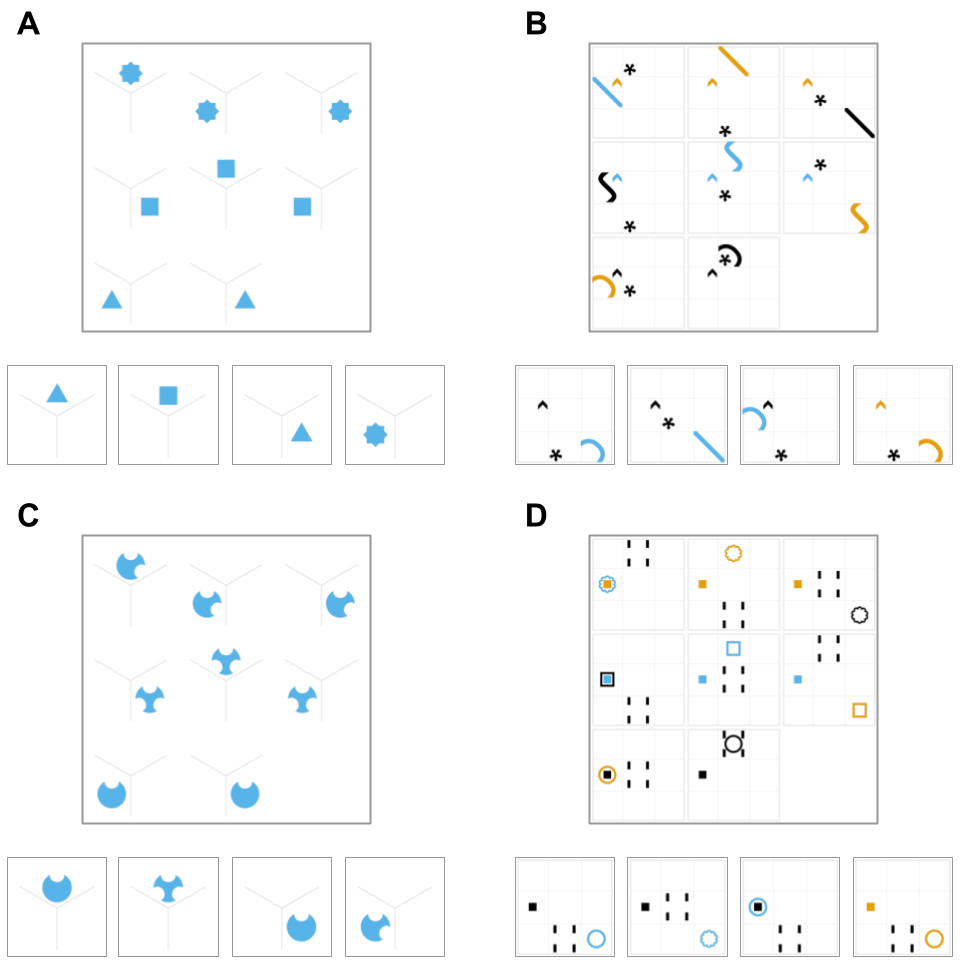
\includegraphics[width=1.0\textwidth]{figures/fig00.png}
\caption{\label{fig:fig00} Example items from the MaRs-IB. (A) A simple item containing a single feature and one relation change (i.e. only the colour changes). (B) A harder item containing three features and six relation changes. In both panels, the first option is the correct solution.}
\end{figure}

\begin{figure}
\centering
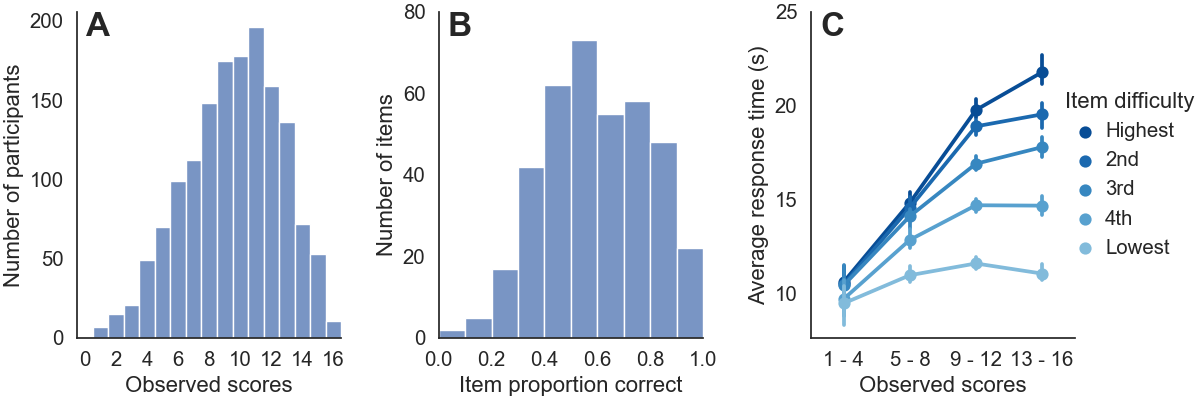
\includegraphics[width=1.0\textwidth]{figures/fig01.png}
\caption{\label{fig:fig01}Summary of performance on the MaRs-IB items. (A) The distribution of total scores across all 1501 participants. (B) The distribution of proportion correct responses across all 384 items. (C) The distribution of participants' median response times across items broken down by participants' total scores and item difficulty (one minus proportion correct responses). Error bars indicate bootstrapped 95\% confidence intervals around the mean.}
\end{figure}
 
\begin{figure}
\centering
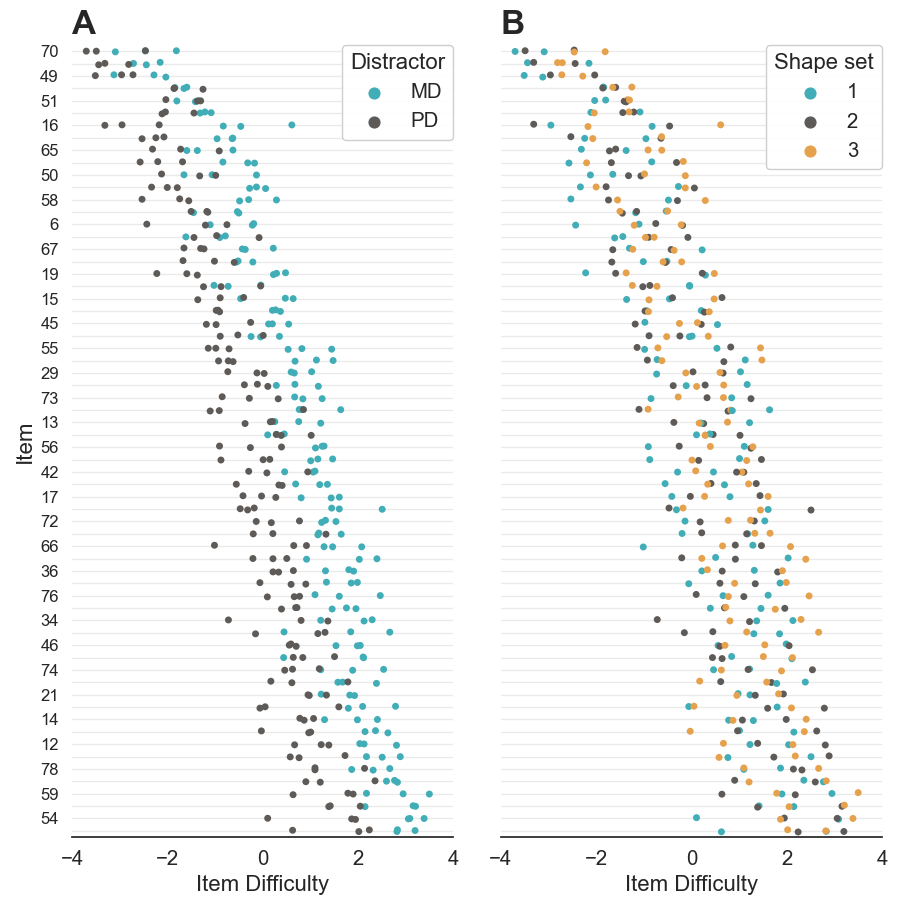
\includegraphics[width=1.0\textwidth]{figures/fig02.png}
\caption{\label{fig:fig02}Results from the test assembly of three parallel MaRs-IB short form (SF) measures. (A) The psychometric properties of the items selected for each form, compared to all remaining items. Points represent the posterior means of the item difficulty and discrimination  parameters. (B) The test characteristic curves (TCCs) for each short form. The degree of overlap highlights the similarity of expected scores for each test form. (C) The test information functions (TIFs) for each short form. The degree of overlap highlights the similarity of reliability for each test form.}
\end{figure}

\begin{figure}
\centering
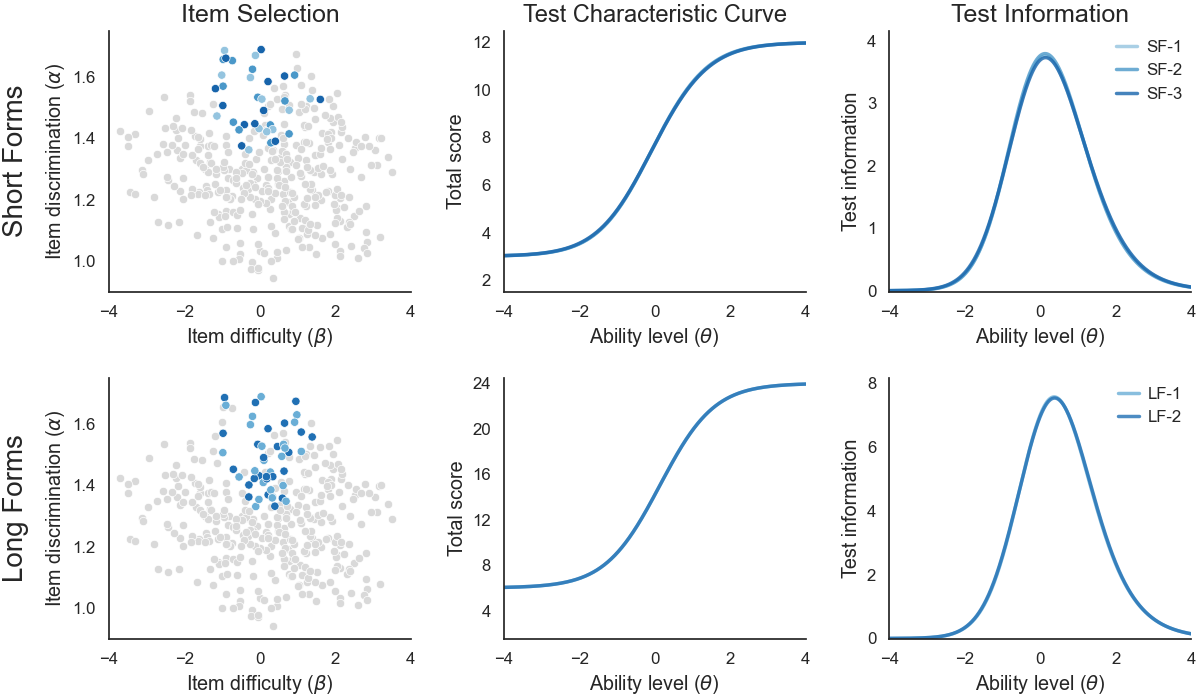
\includegraphics[width=1.0\textwidth]{figures/fig03.png}
\caption{\label{fig:fig03}The joint distribution of total scores on the MaRs-IB short form and abbreviated Raven's progressive matrices (RPM) measures. The distribution of observed scores for each measure are shown in the margins.}
\end{figure}

\end{document}
